\documentclass[10pt,aspectratio=169]{beamer}
\usetheme{metropolis}
\usepackage{appendixnumberbeamer}
\usepackage{booktabs}
\usepackage{graphicx}
\usepackage{tikz}
\usepackage{amsmath}
\usepackage{xcolor}

% Define NHS colors
\definecolor{nhsblue}{RGB}{0,94,184}
\definecolor{nhsdarkblue}{RGB}{0,48,135}
\definecolor{nhsgreen}{RGB}{0,177,64}
\definecolor{nhsred}{RGB}{218,41,28}

% Set theme colors
\setbeamercolor{frametitle}{bg=nhsblue,fg=white}
\setbeamercolor{progress bar}{fg=nhsgreen}
\setbeamercolor{title separator}{fg=nhsblue}
\setbeamercolor{alerted text}{fg=nhsred}

\metroset{progressbar=frametitle,sectionpage=progressbar,numbering=fraction}

\title{Agent-Based Simulation for Neovascular AMD Treatment Planning}
\subtitle{Optimizing Anti-VEGF Therapy Protocols in the NHS}
\author{Your Name\\Consultant Ophthalmologist}
\institute{Your NHS Trust}
\date{\today}

\begin{document}

\maketitle

% Acknowledgments in title frame note
\begin{frame}{Acknowledgments}
\begin{itemize}
    \item Health Service Modelling Associates (HSMA) team
    \item Finance Director and IT Director
    \item NHS England Pharmacy \& Clinical Support Team
\end{itemize}
\end{frame}

\section{Understanding Neovascular AMD}

\begin{frame}{What is Neovascular AMD (NAMD)?}
\begin{columns}[T]
\column{0.5\textwidth}
\begin{itemize}
    \item Leading cause of central vision loss
    \item Cannot read or recognize faces
    \item Leads to legal blindness if untreated
    \item Affects quality of life severely
\end{itemize}

\column{0.5\textwidth}
\begin{figure}
    % Placeholder for vision comparison image
    \centering
    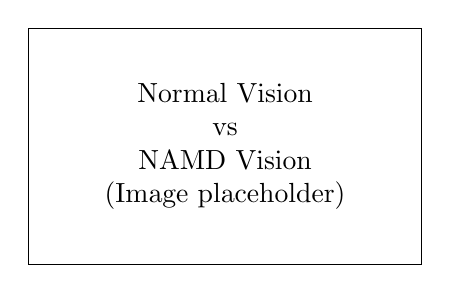
\begin{tikzpicture}
        \node[draw,minimum width=5cm,minimum height=3cm,align=center] {Normal Vision\\vs\\NAMD Vision\\(Image placeholder)};
    \end{tikzpicture}
\end{figure}
\end{columns}
\end{frame}

\begin{frame}{The Biology Behind NAMD}
\begin{columns}[T]
\column{0.6\textwidth}
\textbf{Disease Process:}
\begin{itemize}
    \item Aging eye environment changes
    \item Abnormal blood vessel growth
    \item Leakage, fibrosis, and bleeding
    \item Mediated by VEGF (Vascular Endothelial Growth Factor)
\end{itemize}

\column{0.4\textwidth}
\begin{figure}
    \centering
    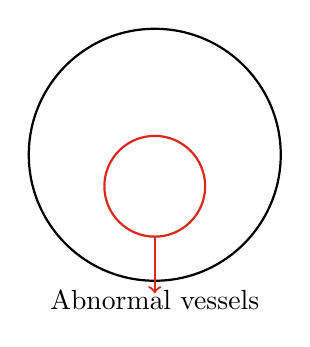
\begin{tikzpicture}[scale=0.8]
        % Simple eye diagram
        \draw[thick] (0,0) circle (2cm);
        \draw[thick,nhsred] (0,-0.5) circle (0.8cm);
        \node at (0,-2.3) {Abnormal vessels};
        \draw[->,thick,nhsred] (0,-1.3) -- (0,-2.2);
    \end{tikzpicture}
\end{figure}
\end{columns}
\end{frame}

\begin{frame}{Revolutionary Treatment: Anti-VEGF Therapy}
\begin{columns}[T]
\column{0.6\textwidth}
\textbf{How it works:}
\begin{itemize}
    \item Antibodies bind to VEGF
    \item Remove growth factor from eye
    \item Stop abnormal vessel growth
\end{itemize}

\vspace{0.5cm}
\alert{\textbf{The Challenge:}}
\begin{itemize}
    \item Molecules cleared over time
    \item Requires repeated injections
    \item Optimal frequency unknown
\end{itemize}

\column{0.4\textwidth}
\begin{figure}
    \centering
    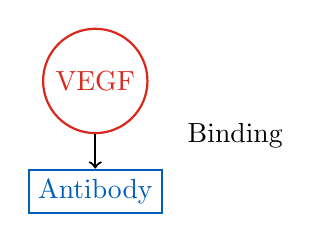
\begin{tikzpicture}[scale=0.7]
        % VEGF binding diagram
        \node[circle,draw,nhsred,thick,minimum size=1cm] (vegf) at (0,2) {VEGF};
        \node[draw,nhsblue,thick,minimum width=1.5cm] (ab) at (0,0) {Antibody};
        \draw[->,thick] (vegf) -- (ab);
        \node[right] at (1.5,1) {Binding};
    \end{tikzpicture}
\end{figure}
\end{columns}
\end{frame}

\begin{frame}{Real-World Treatment Challenges}
\begin{alertblock}{Why Patients Stop Treatment}
\begin{itemize}
    \item \textbf{Mortality}: Elderly population (average age 80+)
    \item \textbf{Frailty}: Too unwell to attend monthly appointments
    \item \textbf{Treatment failure}: Vision deteriorates despite therapy
    \item \textbf{NHS capacity}: Limited appointment availability
\end{itemize}
\end{alertblock}

\begin{block}{Discontinuation Rates}
\begin{itemize}
    \item Year 1: 10-15\% stop treatment
    \item Year 2: Additional 10-15\%
    \item By Year 5: Only 50-60\% still on treatment
\end{itemize}
\end{block}

\centering
\textbf{Critical Question: How do we optimize treatment for those who remain?}
\end{frame}

\section{The Cost Challenge}

\begin{frame}{NHS Annual Treatment Costs}
\begin{table}
\centering
\begin{tabular}{lrr}
\toprule
Treatment Area & Annual NHS Spend & Patient Numbers \\
\midrule
\alert{Wet AMD (Anti-VEGF)} & \alert{£600-800 million} & 700,000+ total \\
& & 39,800 new/year \\
Cataract Surgery & £320-480 million & 400,000/year \\
Hip Replacement & £500-700 million & 100,000/year \\
\bottomrule
\end{tabular}
\end{table}

\vspace{0.3cm}
\begin{alertblock}{Key Insight: Cost per QALY}
\begin{itemize}
    \item Cataract surgery: £1,964 per QALY (exceptional value)
    \item Hip replacement: £2,128 per QALY (strong value)
    \item \alert{Wet AMD: £58,047 per QALY (3x NICE threshold)}
\end{itemize}
\end{alertblock}

\begin{block}{Current Anti-VEGF Drug Costs (2024 list prices)}
\begin{itemize}
    \item Aflibercept (Eylea): £816 per injection
    \item Generic aflibercept: Coming soon (expected 50\% reduction)
    \item Patients need 8-10 injections year 1, then 4-5/year ongoing
\end{itemize}
\end{block}

\centering
\textbf{Challenge: £1.2-1.5 billion projected cost by 2035}
\end{frame}

\section{Why Model?}

\begin{frame}{The Need for Modeling}
\begin{columns}[T]
\column{0.5\textwidth}
\textbf{Current Challenges:}
\begin{itemize}
    \item Treatment controversies
    \item Limited real-world data
    \item Complex patient pathways
    \item Resource constraints
\end{itemize}

\column{0.5\textwidth}
\textbf{Modeling Benefits:}
\begin{itemize}
    \item Explore treatment strategies
    \item Clarify outcome measures
    \item Predict resource needs
    \item Evidence-based decisions
\end{itemize}
\end{columns}
\end{frame}

\begin{frame}{Two Modeling Approaches}
\begin{columns}[T]
\column{0.5\textwidth}
\textbf{Simple Approach (NHS England):}
\begin{itemize}
    \item Excel spreadsheet
    \item "Best guess" parameters
    \item Average patient behavior
    \item Quick but limited insights
\end{itemize}

\column{0.5\textwidth}
\textbf{Our Approach (Agent-Based):}
\begin{itemize}
    \item Individual patient simulation
    \item Build from known parameters
    \item Probabilistic events
    \item Rich, detailed insights
\end{itemize}
\end{columns}

\vspace{0.5cm}
\centering
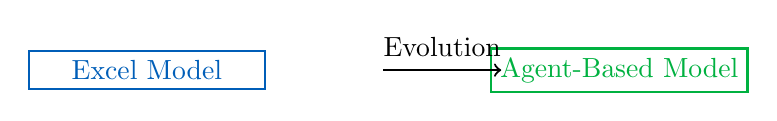
\begin{tikzpicture}
    \node[draw,nhsblue,thick,minimum width=3cm] at (0,0) {Excel Model};
    \node[draw,nhsgreen,thick,minimum width=3cm] at (6,0) {Agent-Based Model};
    \draw[->,thick] (3,0) -- (4.5,0);
    \node at (3.75,0.3) {Evolution};
\end{tikzpicture}
\end{frame}

\begin{frame}{Real-World Complexity in Our Simulation}
\begin{alertblock}{What Simple Models Miss}
\begin{columns}[T]
\column{0.5\textwidth}
\textbf{Simple Models Assume:}
\begin{itemize}
    \item All patients start with same vision
    \item Perfect treatment adherence
    \item No appointment delays
    \item Uniform response to treatment
\end{itemize}

\column{0.5\textwidth}
\textbf{Our Simulation Includes:}
\begin{itemize}
    \item \alert{Vision distribution at baseline}
    \item \alert{Real discontinuation patterns}
    \item \alert{Treatment gaps and delays}
    \item Individual patient trajectories
\end{itemize}
\end{columns}
\end{alertblock}

\begin{block}{Why This Matters}
\begin{itemize}
    \item Captures NHS capacity constraints
    \item Models actual patient populations
    \item Predicts realistic outcomes
    \item Enables better resource planning
\end{itemize}
\end{block}

\centering
\textbf{Result: Evidence-based insights, not theoretical averages}
\end{frame}

\section{Our Solution}

\begin{frame}{Application Architecture}
\centering
\textbf{Four Key Modules:}

\vspace{0.5cm}
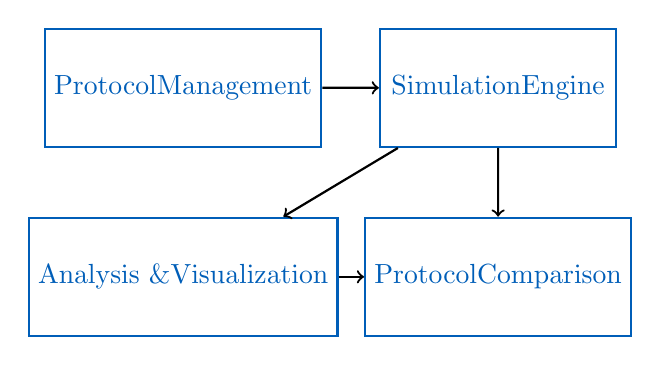
\begin{tikzpicture}[scale=0.8]
    \node[draw,nhsblue,thick,minimum width=3cm,minimum height=1.5cm] (proto) at (0,3) {Protocol\\Management};
    \node[draw,nhsblue,thick,minimum width=3cm,minimum height=1.5cm] (sim) at (5,3) {Simulation\\Engine};
    \node[draw,nhsblue,thick,minimum width=3cm,minimum height=1.5cm] (analysis) at (0,0) {Analysis \&\\Visualization};
    \node[draw,nhsblue,thick,minimum width=3cm,minimum height=1.5cm] (compare) at (5,0) {Protocol\\Comparison};
    
    \draw[->,thick] (proto) -- (sim);
    \draw[->,thick] (sim) -- (analysis);
    \draw[->,thick] (sim) -- (compare);
    \draw[->,thick] (analysis) -- (compare);
\end{tikzpicture}

\vspace{0.5cm}
\alert{Next: Live demonstration of the application}
\end{frame}

% Placeholder for screen recording section
\begin{frame}{Live Demonstration}
\centering
\Large
[Switch to Screen Recording]

\normalsize
\vspace{1cm}
Demonstration includes:
\begin{itemize}
    \item Loading treatment protocols
    \item Running 1000-patient simulation
    \item Exploring patient journeys
    \item Visualizing population outcomes
    \item Comparing different protocols
\end{itemize}
\end{frame}

\section{Key Insights}

\begin{frame}{What We've Learned}
\begin{columns}[T]
\column{0.5\textwidth}
\textbf{Model Reveals:}
\begin{itemize}
    \item Treatment pattern impacts
    \item Resource utilization peaks
    \item Patient outcome distributions
    \item Protocol efficiency metrics
\end{itemize}

\column{0.5\textwidth}
\textbf{Enables:}
\begin{itemize}
    \item Evidence-based protocols
    \item Capacity planning
    \item Cost-effectiveness analysis
    \item Commissioning decisions
\end{itemize}
\end{columns}

\vspace{0.5cm}
\begin{alertblock}{Future Development}
Cost calculator module in development for full economic analysis
\end{alertblock}
\end{frame}

\begin{frame}{Thank You}
\centering
\Large
Questions?

\vspace{1cm}
\normalsize
\textbf{Contact:}\\
your.email@nhs.net

\vspace{0.5cm}
\textbf{Project Repository:}\\
\url{https://github.com/yourusername/namd-simulation}

\vspace{0.5cm}
\textbf{Acknowledgments:}\\
HSMA Team | NHS England | Trust Leadership
\end{frame}

\end{document}